\documentclass[12pt]{article}

% margin left and right with \setlength{\itemindent}{-.5in} %
\usepackage{enumitem}

% leave out section numbers in subsection numbering %
\usepackage[T1]{fontenc}
\renewcommand*\thesubsection{\arabic{subsection}}

% include Roman numerals for sections %
\renewcommand{\thesection}{\Roman{section}}
%Roman numerals for subsections like this \renewcommand{\thesubsection}{\Roman{subsection}}%
% include the package of the color%
\usepackage[usenames, dvipsnames]{color}
\usepackage[english]{babel}
\usepackage[utf8x]{inputenc}
\usepackage{amsmath}
\usepackage{graphicx}
\usepackage{subfiles}

%define your own color %
\definecolor{mygray}{gray}{0.9}
\begin{document}
	\listoffigures
	\title{Chapter 1 : General Project Presentation}
	\maketitle

	\section{Host Company Presentation}
	
	\subsection{Presentation of MASS Analytics}
	MASS Analytics, a Tunisian start-up founded in 2012, is the first and only independent Marketing Mix Modeling (MMM) agency in the MENA region. MASS Analytics’ core competency is the deep analysis and understanding of what impacts the consumer's path to purchase to make companies more effective with their marketing budget.
	\\
	\\
	It was founded by \textbf{Dr. Ramla Jarrar } ( Chief Executive Officer ),  \textbf{Dr. Firas Jabloun } (Chief Technology Officer), \textbf{Nadia Bouzguenda} (Business Development Director) \& \textbf{Rafal Kozlowski} (Director). They brought the essence of more than 20 cumulative years of experience in marketing effectiveness \& technology services at the international level to the creation of MASS-Analytics. \cite{ref1}
	\\
	\\
	\begin{figure}[h]
	\centering
	
\includegraphics[width=0.15\textwidth]{Mass_logo.png}
	\caption{Mass-Analytics logo}
    \end{figure}
	\subsection{Services}
	\begin{itemize}
		\item \textbf{MassTer Software :} MASS Analytics has been developing internally its own Marketing Mix Modeling Software ``MassTer''. It is one of the most powerful Marketing Mix Modeling software products/solutions in the world and comes in three packages: standard, professional , and premium. It provides the user with a powerful Modeling platform coupled with a comprehensive data visualization capability to help understand the relationship between different variables and measure their impact on business performance.
		\begin{figure}[h]
			\centering
			
\includegraphics[width=0.2\textwidth]{massTer_logo.png}
			\caption{MassTer Software logo}
		\end{figure}
		
		\item \textbf{Training and Consultancy :} MASS Analytics runs specific courses and training sessions on advanced predictive modeling (log linear, nested modeling, fixed effect modeling…), budget optimization and return on Investment calculation. It also offers its clients coaching sessions to help improve their marketing analytics process and project delivery.
	\end{itemize}
\vspace{66mm}
	\subsection{Customers}
	
		\begin{figure}[h]
		\centering
		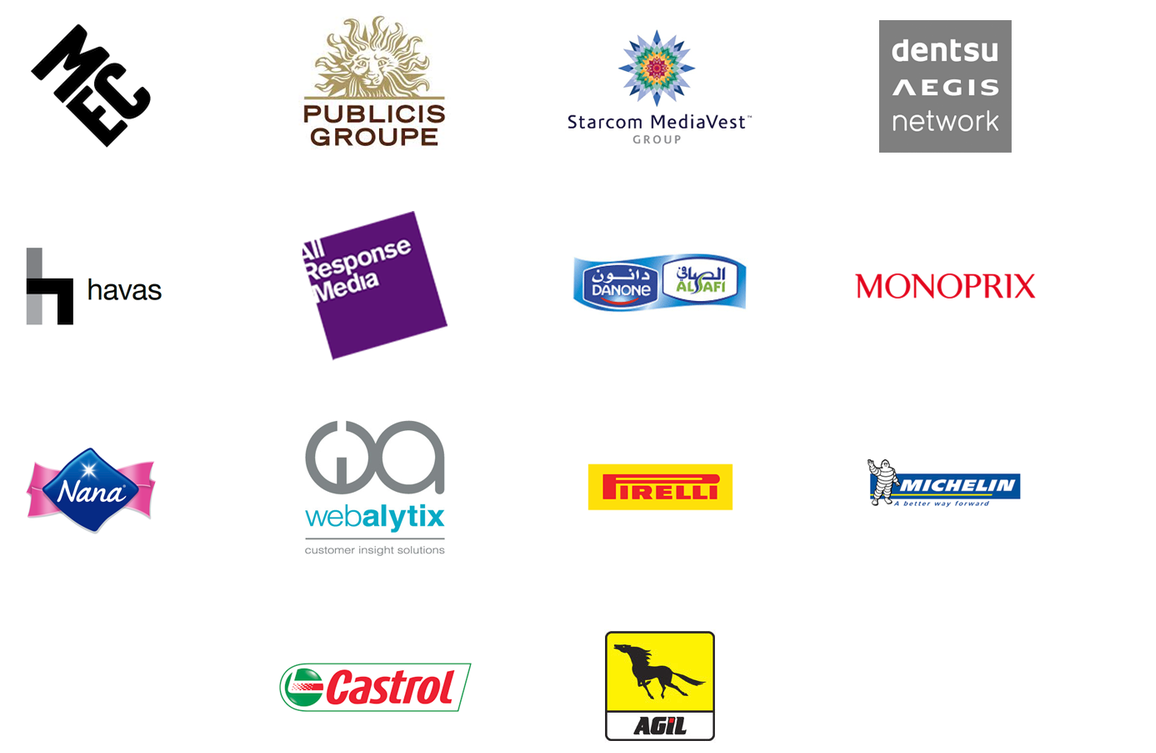
\includegraphics[width=0.8\textwidth]{customers_logo.png}
		\caption{Some of MASS Analytics’ customers logo}
	\end{figure}
	\section{Project Presentation}
	
	\subsection{Context}
	As part of its software development and consulting activities, oriented towards the business of Marketing Mix Modelling (MMM), Mass-Analytics is always looking to offer its customers products that are the most efficient and smart. Thus, It seeking to provide innovative services that satisfied the different needs of customers based on new technologies.
	\\
	\\
	In this context, this project entitled \textbf{MassTer Insight SaaS} was offered to me by Mass-Analytics as part of a graduation project to obtain the national diploma of computer engineer.      
	\subsection{Objectives}
	The main objective of this project is to develop MassTer Insight from the exiting Desktop solution to a SaaS.
	\\
	\\
	We are in charge to keep the same business logic of the desktop solution, but offered to the customers in cloud SaaS version with Security guaranteed,  high perform in term of Speed, Visualization, Graphics, Design .
	\subsection{Problematic}
	Today all the companies move to cloud, they are tend to by their softwares through cloud SaaS, for more reasons : one amongst the reason is security, when you offer an executable software, this one is threaten by the crack, also an executable requires sometimes to take care of your resources needs, an important RAM, CPU, and more. Almost the executable save data locally which is a very bad way to stock data, it is possible to loose these data once the hard disk is defect by an external effect or even internal. we don't need to inform the customer for each updates to keep installing our software, once he/she connect on the web application he/she got the last version without any process of installation.  
	\\
	\\
	That's what we care about, our current solution Masster Insight desktop is threaten by the crack, may will be heavy on machine with smaller resources, works only on pc. it requires the process of installation wasted time.

	\section{Methodology}
	The choice of the methodology is an important step in software development since it grants formalizing the preliminary steps when establishing a system in pursuance of the client’s requirements.
	The scrum , an approach that is part of the Agile movement, was used when carrying out this project.
	
	\newpage
	
	\section{Software Development Life Cycle}
	We chosen the \textbf{Iterative Model }as Software Development Life cycle (SDLC).
	\\
	\\
	This model turns the process of development in cyclic manner repeating very step after every cycle of SDLC process. 
	
	\begin{figure}[h]
		\centering
		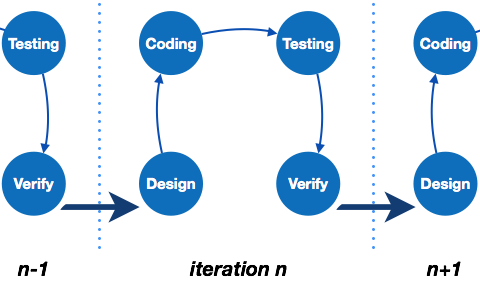
\includegraphics[width=1\textwidth]{sdlc_iterative.png}
		\caption{sdlc iterative}
	\end{figure}  

	\newpage

	\section{Software Development Process}
	Test-driven development (TDD) is a techniques of implementation code, starts with developing test for each features. 
	\\
	\\
	The developer writes a little test code and then implements the business, in the traditional method, the test comes from the code, but in TDD the business code is submissive to tests then it is corrected until the tests are validated. 
	
		\begin{figure}[h]
		\centering
		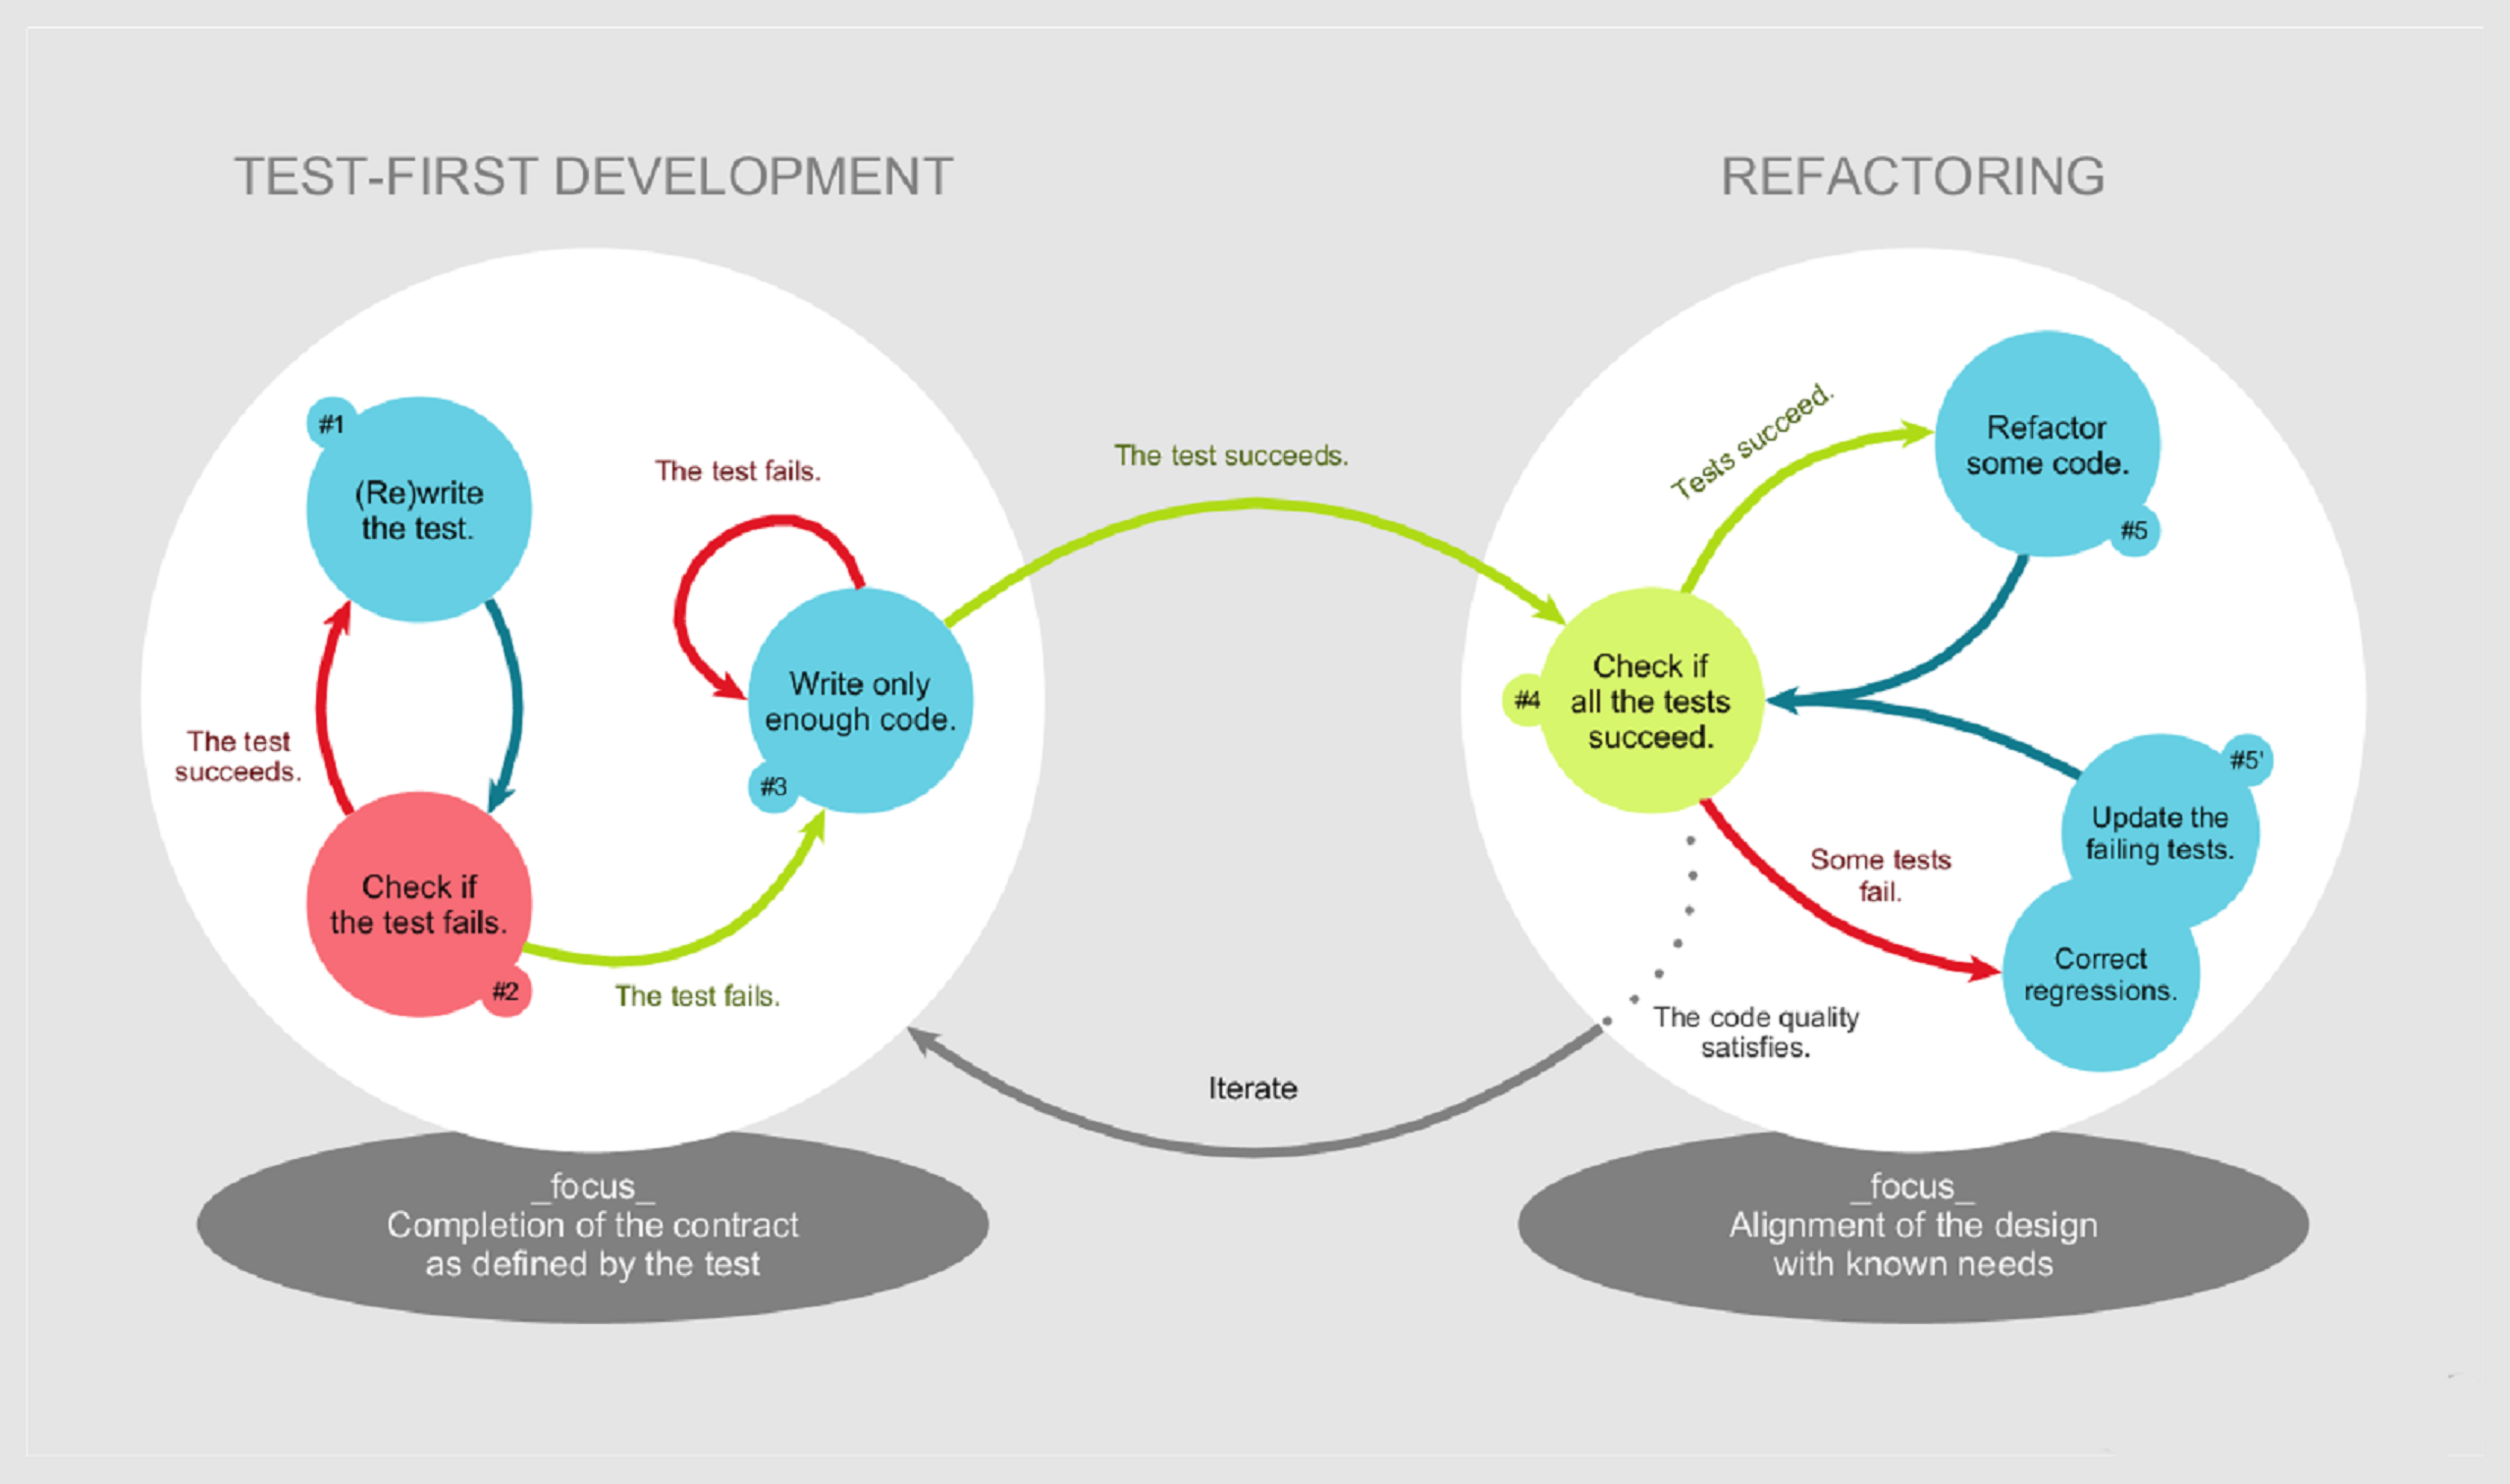
\includegraphics[width=1\textwidth]{TDD_Global_Lifecycle.png}
		\caption{TDD Global Lifecycle}
	\end{figure}   
	\section{Existing Presentation}
	\textbf{MassTer Insight Desktop Application} is an easy to use software that allows you to run simulation scenarios and allocate your budget optimally across Regions, Products, Channels and Periods. It tells you how much budget to spend on every single media channel and in which period, given a complex modeling structure. It will helps you to benefit from your Marketing Mix Modeling projects [1]. 

	\section{Conclusion}
	This chapter was a presentation of the hosting company, its services, and clients. The problematic of the project was also highlighted, along with the proposed solution and the methodology followed while carrying out the project.
	\bibliographystyle{plain}
	\bibliography{webo} 
\end{document}
